\documentclass[letterpaper, 11pt]{scrartcl}
\usepackage[T1]{fontenc}
\usepackage[utf8]{inputenc}

\usepackage{times}
\usepackage{amssymb}

% lucimono is custom package I made ages ago for the Lucida Mono font I purchased.
%  use luximono on systems without it.
\newif\ifmyhaslucimono
\makeatletter
\let\originput\@@input
\makeatother

\IfFileExists{lucimono.sty}{\myhaslucimonotrue}{\myhaslucimonofalse}

\ifmyhaslucimono
\usepackage[scaled=0.8]{lucimono}
\else
\usepackage[scaled=0.8]{luximono}
\fi

\usepackage{upquote}
\usepackage{footnote}
\usepackage{subfig}
\usepackage{enumitem}
\setlist{noitemsep}
\usepackage[section]{placeins}
\usepackage{tikz}

% put url in footnote for hyperlinks
\newcommand{\myhref}[2]{\href{#1}{#2}\footnote{\url{#1}}}

% use the section numbering scheme also used in official proposal template
\renewcommand{\thesubsection}{\thesection.\Alph{subsection}}

% define emoji strings
\newcommand{\emojipedia}[1]{$\vcenter{\hbox{\includegraphics[height=\baselineskip]{emojipedia/#1}}}$}
%
\newcommand{\brainemoji}{\textbf{BRAIN} \emojipedia{brain_1f9e0.png}}
\newcommand{\jigsawemoji}{\textbf{JIGSAW} \emojipedia{jigsaw-puzzle-piece_1f9e9.png}}
\newcommand{\rainbow}{\textbf{RAINBOW} \emojipedia{rainbow_1f308.png}}
\newcommand{\prideflag}{\textbf{RAINBOW FLAG} \emojipedia{rainbow-flag_1f3f3-fe0f-200d-1f308.png}}
\newcommand{\nerdface}{\textbf{NERDFACE} \emojipedia{nerd-face_1f913.png}}
\newcommand{\goldheart}{\textbf{YELLOW HEART} \emojipedia{yellow-heart_1f49b.png}}
\newcommand{\infinityemoji}{$\circledast{}$ \textbf{INFINITY} \emojipedia{permanent-paper-sign_267e.png}}

\usepackage[unicode,colorlinks,linkcolor=violet,urlcolor=blue,pdftitle=Proposal\ for\ NEURODIVERSITY\ Emojis]{hyperref}

\title{Proposal for NEURODIVERSITY Emojis}
\author{Alice Wonder}

\begin{document}

\maketitle

\begin{abstract}
I am proposing an emoji sequence for \textbf{NEURODIVERSITY}

\begin{figure}[h!]
\caption{Neurodiversity Emoji Concept Art}
\centering
  \subfloat[Option A: Rainbow Brain]{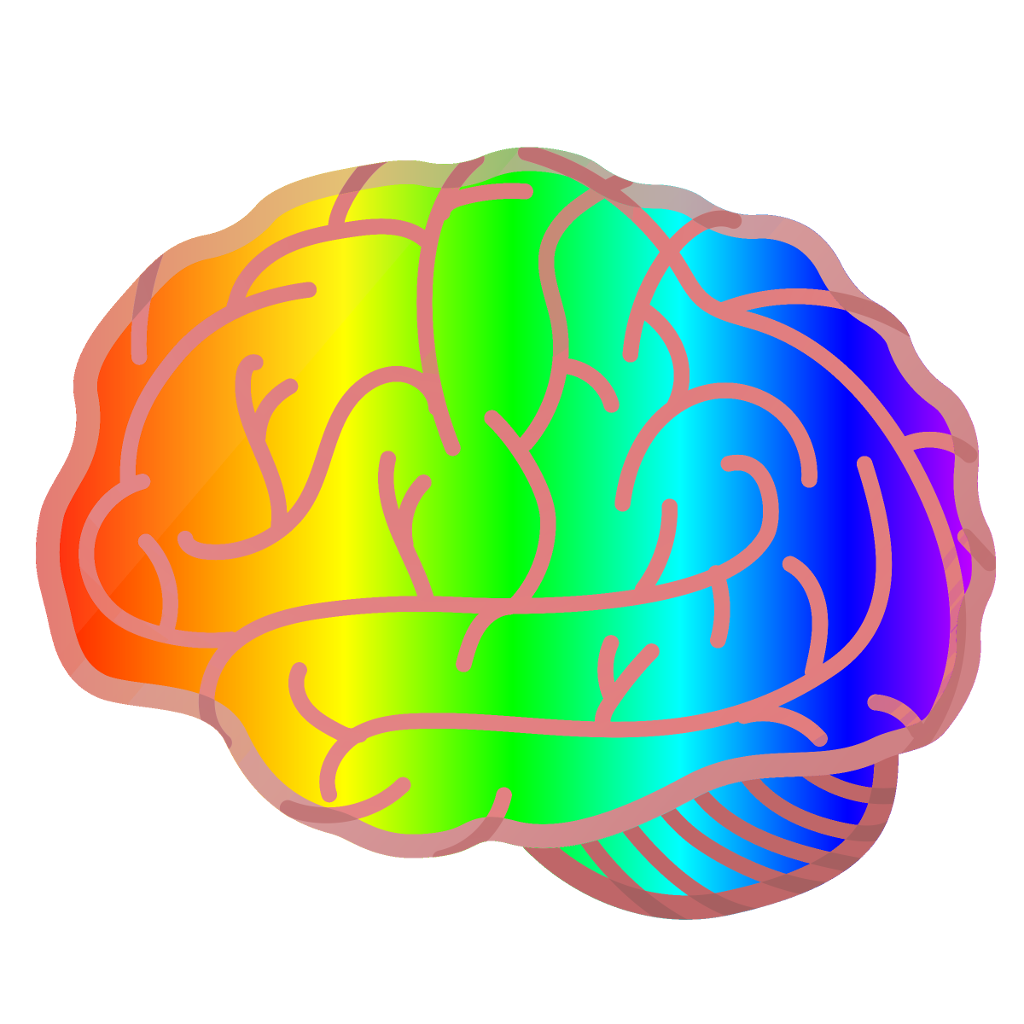
\includegraphics[width=0.333\textwidth]{neurodiversity.png}}
  \qquad
  \subfloat[Option B: Rainbow Infinity Loop]{
\includegraphics[width=0.333\textwidth]{SpectrumInfinity.png}}
%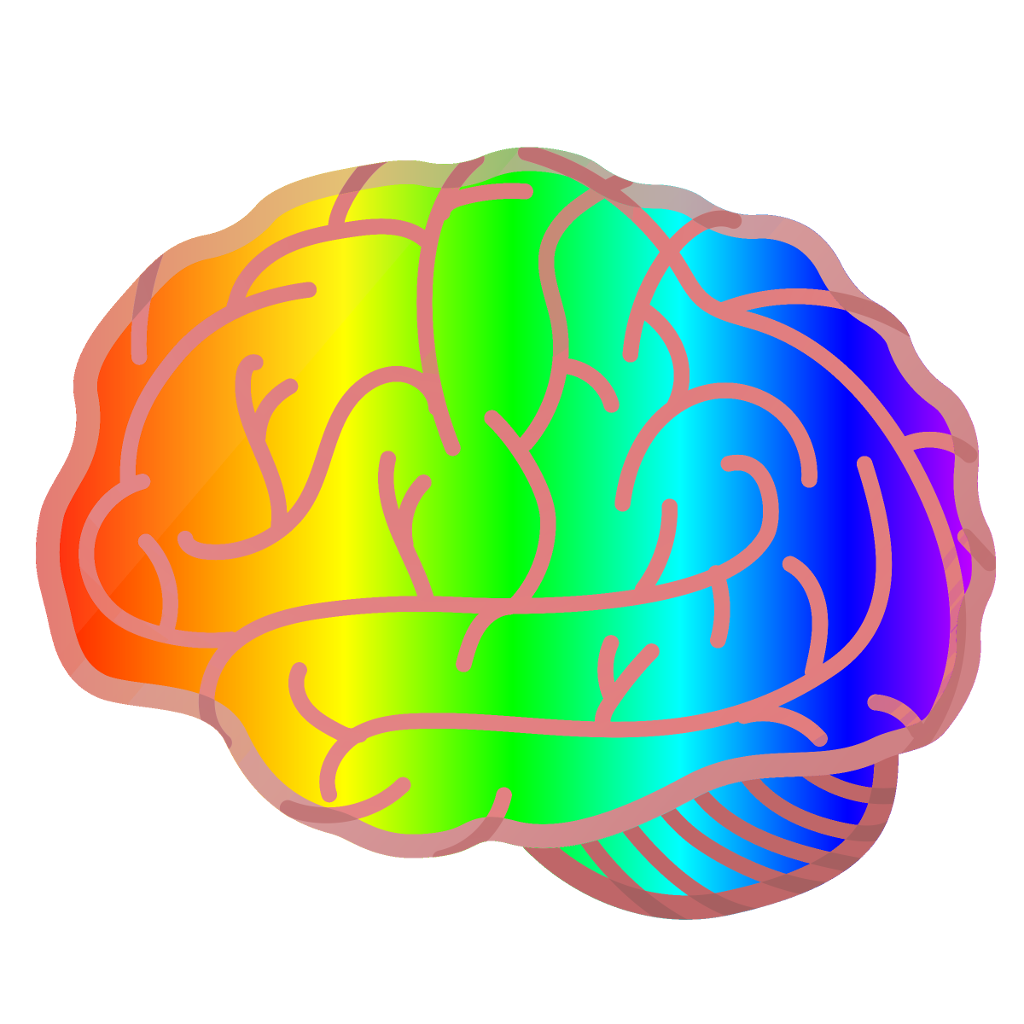
\includegraphics[width=0.333\textwidth]{neurodiversity.png}
\label{fig:neurodiversity}
\end{figure}

This is a very rough draft and is subject to radical change.

Autism (often referred to as Autism Spectrum Disorder) refers to a spectrum of
characteristics that are the result of a neurologically
atypical brain. Typical characteristics include repetitive behaviors, differences in language
processing, difficulty in social interactions, and differences in how emotions and
empathy are expressed.

The center for disease control estimates that roughly 1 in 59 eight year olds is
autistic\footnote{\url{https://www.autism-society.org/news/2018-cdc-autism-incidence-rate-statement-from-the-autism-society/}}.
Generally boys are more likely to be diagnosed as autistic than girls, though that
may be due to differences in social constructs regarding the expected behavior of
boys and girls resulting in a higher percentage of autistic girls going undiagnosed.

As online social networking makes it easier for autistic individuals to find each
other, our positive identity as a demographic rather than a negative identity as a
disorder is starting to grow.

We believe an emoji to express our neurodiverse identity, an emoji chosen by our
community, is both warranted and will help us continue to identify each other and
grow as a community, enabling us to receive the important peer support we often
lack from society at large.

The primary difference between those who are autistic and those who are not is in
how our brain works. A rainbow represents the full spectrum of visible light. We
believe a rainbow brain is a logical representation of the neurodiverse spectrum that
makes up our community.

Many members of the Neurodiverse community already identify with either the rainbow
brain or the rainbow infinity loop shown in figure~\ref{fig:neurodiversity}.

We respectfully request that one or both be added to the official Emoji list.
\end{abstract}


\section*{Conventions}

This proposal is attempting to follow the proposal guidelines specified at
\url{https://unicode.org/emoji/proposals.html} using the same section numbering
scheme used in the form specification there.

Section Six, \textit{`Other Information'} in the proposal form template, has been renamed to
\textit{`Selection Factors --- Special Consideration'}.

Sometimes I over-explain thing. It is an autism trait often known as `data dumping' and
is often frowned upon by those who are neurotypical. I have tried very hard not to do
it here, but I ask for an ounce of grace if and when I over-explain something.

\subsection*{Existing Emojis}

Existing emojis used in this document will be referenced using upper case bold text for the CLDR short name
followed by an image of the emoji.

Unfortunately \TeX{}Live does not directly support color emoji fonts. I was forced to
use a hack that inserts the emojis as images.

I apologize if that screws up automated software that generates emoji use statistics.
\LaTeX{} is the only word processor I ever was able to figure out how to get it to do
what I want. Well, um,
until now when I wanted to insert emojis... ;)

\subsection*{Hyperlinks}

Hyperlinks where the text of the hyperlink is not the URL will have the URL specified
in a footnote.

\subsection*{Figures}

With the exception of the concept art for the proposed emojis at the top of
this document, all figures appear in Appendix~\ref{apx:figures}.
This makes it easier to note that the images in the figures are used under the Fair
Use doctrine so that it is very clear the copyright to those images does not belong
to me. I like to be very clear
when it comes to intellectual property.

\subsection*{Community Participation}

I, Alice Wonder, am only a \emph{member} of the Autistic / Neurodiverse community.

This document was created on a
\myhref{https://github.com/AliceWonderMiscreations/NeurodiversityEmoji}{Public Github}
where any member of the community is free to either create issues or submit pull
requests.

Community participation has been sought at both Twitter and Facebook
before submission of this proposal to the Unicode Consortium to make sure this proposal is
congruent with the those the emoji is intended to represent.

Feedback from members of the community on both Twitter and Facebook has been positive. It
is only a very small sampling of the larger community, but I did my best to contact as
many members of the community as I could.


\pagebreak
\tableofcontents
\pagebreak
\listoffigures

\pagebreak

%The parts of the Character Proposal Form
\section{Identification}

\subsection{CLDR short name}
The suggested CLDR short name: \textbf{Neurodiversity}

\subsection{CLDR keywords}
The suggested CLDR keywords: \textbf{Neurodiversity, Neurodiverse, Autism, Autistic, ASD, Asperger}

\section{Images}

The Rainbow Brain concept art in this proposal is based on the Google\textsuperscript{\textregistered}
\myhref{https://www.google.com/get/noto/help/emoji/}{Noto Color Emoji} font.

It is recommended that emoji fonts base their artwork on their existing glyph for
\brainemoji{}. Monochrome versions of the glyph should just use their
monochrome variant of \brainemoji{} ignoring the rainbow modifier the
same way many of them handle skin tone modifiers when in monochrome.

The Rainbow Infinity Loop concept in this proposal is directly taken from
\myhref{https://commons.wikimedia.org/wiki/File:Autism_spectrum_infinity_awareness_symbol.svg}{Wikimedia Commons}
with only a canvas change to make the artwork square. Monochrome versions of the glyph
should \emph{probably} just use a monochrome infinity loop.

\subsection{Zip File}
A zip file containing the concept art can be downloaded from:
\myhref{https://github.com/AliceWonderMiscreations/NeurodiversityEmoji/raw/master/NeurodiversityEmoji.zip}{NeurodiversityEmoji.zip}.

The zip archive contains both opens in the following sizes:

\begin{itemize}
\item 1024x1024
\item 256x256
\item 128x128
\item 72x72
\end{itemize}

The Apache 2.0 license text for the Rainbow Brain option is included in the zip file.

\subsection{License}

The Rainbow Brain concept artwork is a derivative of the Noto Emoji \brainemoji{} glyph
which uses \myhref{https://github.com/googlei18n/noto-emoji/blob/master/LICENSE}{Apache License, version 2.0}.
A copy of that license is included in the zip archive.

The Infinity Loop concept artwork is from
\url{https://commons.wikimedia.org/wiki/File:Autism_spectrum_infinity_awareness_symbol.svg}
where it is specified as belonging in the public domain.

\subsection{Document}

The form for Emoji Proposals specifies that images for the proposed emoji be included at
the top of this document in both 18x18 and 72x72 pixels.

The zip archive contains the concept art in 1024x1024, 256x256, 128x128, and 72x72. An 18x18 sample
is not included, that size does not make sense, especially when so many devices have a pixel
density of 2:1 or greater.

With all due respect, that part of the `Form for Emoji Proposals' needs to be modified. I do
not even really understand what it is after, and several example proposals I looked at did
not adhere to the text of that guideline. See the
\myhref{http://www.unicode.org/L2/L2016/16279-person-meditating.pdf}{\textbf{PERSON MEDITATING}}
sample proposal. The images there do not include 18x18 pixel images.

Is it possible that 18 point and 72 point is what was intended? Those are common font sizes.
However many (most?) emojis are not even remotely recognizable at 18 pixels by 18 pixels.


\section{Selection Factors --- Inclusion}

\subsection{Compatibility}
Not applicable.

\subsection{Expected Usage Level}

\subsubsection{Frequency}

A search on Twitter revealed several users using \brainemoji{} emoji or a brain in
their avatar in the context of neurodiversity:
\begin{itemize}
  \item \myhref{https://twitter.com/NeuroRebel}{Neurodivergent Rebel}
  \item \myhref{https://twitter.com/diffbrains}{Different Brains}
\end{itemize}

A search on Twitter for neurodivergent / autism related hashtags revealed several users with a rainbow
infinity loop in their avatar:

\begin{itemize}
  \item \myhref{https://twitter.com/AutisticPriest}{Autistic Priest}
  \item \myhref{https://twitter.com/ChiDeltaWithNOR}{Chris Connor}
  \item \myhref{https://twitter.com/Frances_Larina}{Frances\_Larina}
  \item \myhref{https://twitter.com/meowcarriemeow}{Meow Carrie Meow}
\end{itemize}

A search on Twitter revealed several users using \jigsawemoji{} in the context of autism.

\begin{itemize}
  \item \myhref{https://twitter.com/adspong2015lego}{Adam Spong}
  \item \myhref{https://twitter.com/wjxt4/status/1015279222657617922}{News4JAX Tweet}
  \item \myhref{https://twitter.com/EmiForLove/status/1008835449798975490}{Autistic Pride Day Tweet}
\end{itemize}

It is apparent that users of the Twitter platform do want iconography related to neurodiversity
and autism.


\subsubsection{Multiple Usages}

There is at least one possible use for the color brain emoji beyond neurodiversity.

Brain scans and instructive artwork for brains often use colors to indicate different things,
whether it is neurotypical or not, see figure \ref{fig:brainparts}. It would not be surprising
if some people in the field of neuroscience used this emoji sequence outside of the context
of neurodiversity.


\subsubsection{Use in Sequences}

I believe this is not applicable.

It may be able to add these emojis by using a sequence to describe them, such as how
\rainbow{} is used to as a sequence modifier to create the
\prideflag{} emoji.

The technical details of whether to use sequences to add support for these emojis or define
codepoints is beyond the scope of this proposal, that is a Unicode Consortium decision.

\subsubsection{Breaking New Ground}

These emojis \emph{may} break some new ground.

There currently are not any emojis that exist for the purpose of identifying diversity inside
a person. There are emojis for ethnic differences, gender differences, career differences,
even hair style differences.

Nothing seems to exist for differences in people that are fundamentally internal yet are a
huge part of who they are.

An argument could be made for the \nerdface{} and the
\prideflag{} having broken that ground already.

\subsection{Image Distinctiveness}

A rainbow is frequently used as a visual representation of a spectrum. A rainbow itself is
created by diffraction of white light, allowing our eyes to interpret the individual
wavelengths that make up the visible spectrum of light and see the beautiful diversity that
actually exists within white light that we were unable to perceive without the diffraction of
light.

With the proposed Rainbow Brain emoji, it should not be too difficult for people to figure out
the rainbow is acting as a diversity adjective for the brain.

With the proposed Rainbow Infinity Loop emoji, it may require some context initially for people
not already familiar with the Rainbow Infinity Loop to understand the meaning. The current use
of that pictograph by many users already should allow many to know what it means right away.

A rainbow flag is often used as a symbol of pride by the LGBTQIA and sometimes rainbow colors
and patterns are used outside of the context of a flag to indicate LGBTQIA pride. However the
\prideflag{} is more frequently used for
LGBTQIA pride. I do not believe there will be much confusion.

\subsection{Completeness}

In addition to the Rainbow Brain and the Rainbow Infinity Loop, I am aware of two other pictographs
that are sometimes used to indicate neurodiversity in general and/or autism.

A gold heart is sometimes used to indicate Autistic Unity. I \emph{believe} that falls under the
categorization of furthering a cause, which is specified as an invalid reason to request an emoji.

Those who want to use a gold heart also can already do so using \goldheart{}.

Sometimes a puzzle piece is used to indicate autism specifically. The source of this as a pictograph
for autism is due to the organization Autism Speaks using a puzzle piece is their logo, see
figure~\ref{fig:aspeaks}.

Those who wish to use jigsaw puzzle piece to indicate autism can already do so using \jigsawemoji{}
though I would \emph{personally} recommend against it, as it may result in trademark violation when
the emoji font uses a blue puzzle piece for that codepoint.

\subsection{Frequency Request}

Not Applicable, I do not have any data on how often such an emoji is requested either of the
Unicode Consortium or a Unicode member company.

\section{Selection Factors --- Exclusion}

% so that it starts with f, specify counter value
\setcounter{subsection}{5}

\subsection{Overly Specific}

The emojis proposed here are suitable to indicate all forms of neurodiversity. They are not
overly specific to any particular form of neurodiversity.

\subsection{Open-ended}

The two proposed emojis here are the most frequently used pictographs I have seen to indicate
neurodiversity within the neurodiverse community.

Outside the neurodiverse community, and by some members of the autistic community, a jigsaw
puzzle piece is sometimes used. However the puzzle piece is closely tied to a specific organization
and is in fact a trademark of that organization, making it unsuitable for general use.

\subsection{Already Representable}

Some people are already using \brainemoji{} to represent neurodiversity.
It works for the present but only indicates neurodiversity for those
who already understand the context. Far more often, that emoji is used to indicate intelligence
or thinking.

Some people are already using \jigsawemoji{} to represent autism.
When used in the context of autism it has trademark issues, and it
excludes neurodiversity that is not autistic.

\subsection{Logos, Brands, UI Icons, Specific People, Deities}

To the best of my knowledge, the Rainbow Brain and Rainbow Infinity Loop are not exclusive to
any specific brand or person.

I did find the infinity loop in use with some Tarot card decks, but without rainbow coloring.

The blue puzzle piece that Twitter uses for \jigsawemoji{} however is very
similar to a trademark owned by Autism Speaks. See figure~\ref{fig:aspeaks}. Encouraging the
use of a rainbow colored brain or rainbow infinity loop for neurodiversity would help avoid
trademark issues.

\subsection{Transient}

As awareness of autism and other neurodivergent traits increase, the neurodiversity community
will continue to grow, especially online where our social awkwardness is less of an issue. I
expect we will run out of IPv6 address space long before these emojis are no longer of value...

\subsection{Faulty Comparison}

I do not believe this is applicable.

\subsection{Exact Images}

An exact image is not needed for either of these proposed emojis. Emoji font creators have plenty
of artistic license when creating the glyphs to represent them.

\section{Sort Location}

\subsection{Category}

Within the existing category list, this emoji sequence would be a best fit within the
`Body' category.

\subsection{Comes After}

Within the `Body' category, this emoji sequence would be a best fit after the
\textbf{BRAIN} \texttt{U+1F9E0} emoji this sequence is a variant of.

\section{Selection Factors --- Special Consideration}

The emoji \textbf{JIGSAW} \texttt{U+1F9E9} was recently added to the Unicode Emoji list.

The organization \myhref{https://www.autismspeaks.org/}{Autism Speaks} uses a blue puzzle
piece for their logo, see figure~\ref{fig:aspeaks}. Twitter uses a very similar blue
puzzle piece for the \textbf{JIGSAW} emoji, see figure~\ref{fig:twitterJigsaw}

The two are very similar and there is some considerable fear that people outside of the
autism community will start to use that emoji when referencing autism.

Within the autism community (people who are actually autistic themselves) there is a lot of
resentment towards that particular group as well as resentment towards using a puzzle piece
to represent us.

For information on why many (though admittedly not all) within the autistic community dislike
the Autism Speaks organization, see
\myhref{https://neurodivergentrebel.com/2018/03/14/why-autistic-people-generally-dislike-autism-speaks/}{Why Autistic People Generally Dislike Autism Speaks}.

For information on why many within the autistic community do not want to be represented by a
puzzle piece, see
\myhref{https://learnfromautistics.com/the-problem-with-the-autism-puzzle-piece/}{The Problem with the Autism Puzzle Piece}.

Whether or not that organization deserves that resentment from us though is not the issue.
Regardless of those things, it is not a good idea for an emoji that is very close to the
trademark of a specific autism related organization to be used for autism in the general
sense.

The proposed \textbf{NEURODIVERSITY} emoji would give an alternative that will not be confused
with the trademark of a specific autism related organization while at the same time giving our
community an emoji to use that we specifically chose to identify with.

The proposed \textbf{NEURODIVERSITY} emoji avoids the potential misuse of the \textbf{JIGSAW} \texttt{U+1F9E9}
emoji in the autism context it was not intended for.


%end parts of the Character Proposal Form

\pagebreak
\appendix
\section{Figures}
\label{apx:figures}

\begin{figure}[ht]
\caption{Autism Speaks Logo}
\centering

\includegraphics[width=0.333\textwidth]{aspeaks}
\label{fig:aspeaks}
\end{figure}

\begin{figure}[ht]
\caption{Twitter Jigsaw Emoji}
\centering

\includegraphics[width=0.2\textwidth]{twitterJigsaw}
\label{fig:twitterJigsaw}
\end{figure}

\begin{figure}[ht]
\caption{Autistic Twitter User with Brain Emoji. Notice the brain on her shirt is rainbow.}
\centering

\includegraphics[width=0.3\textwidth]{rebel.png}
\label{fig:rebel}
\end{figure}

\begin{figure}[ht]
\caption{Autistic Twitter User with Puzzle Piece. Personal information about the user intentionally obfuscated.}
\centering
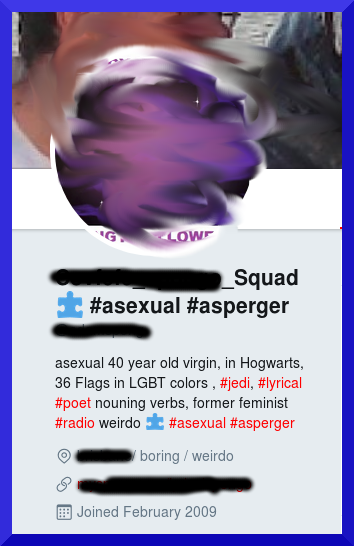
\includegraphics[width=0.3\textwidth]{covfefe.png}
\label{fig:covfefe}
\end{figure}

\begin{figure}[ht]
\caption{Instructive drawing of brain using multiple colors}
\centering
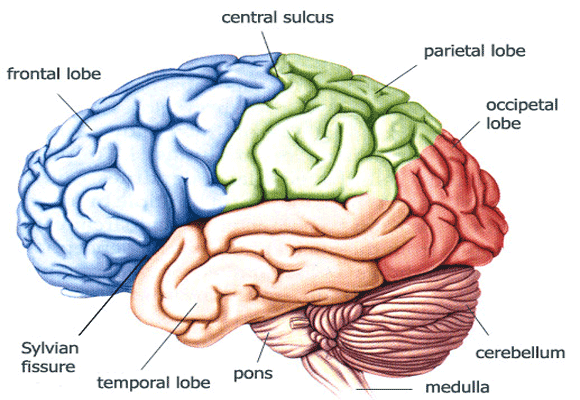
\includegraphics[width=0.5\textwidth]{brainparts.png}
\label{fig:brainparts}
\end{figure}

\begin{figure}[ht]
\caption{Rainbow Infinity Loop}
\centering
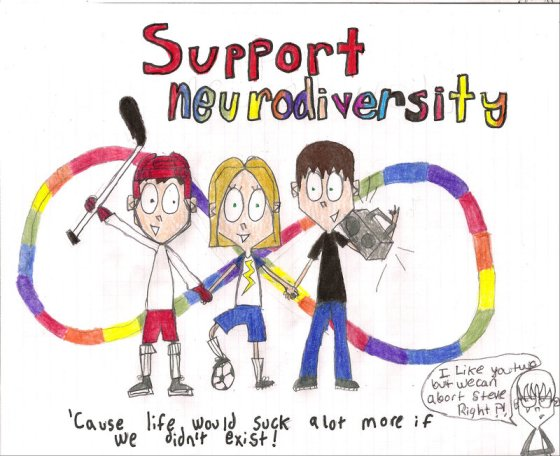
\includegraphics[width=0.5\textwidth]{infinity.jpg}
\label{fig:infinity}
\end{figure}

\pagebreak
\section{acknowledgement}

The following people either directly or indirectly contributed to the creation of this
proposal. Those who I know are members of the neurodiversity community are listed first
in alphabetical order. Those who I do not know are memberd of the neurodiversity community
(though it is possible they are) are listed second in alphabetical order.

\begin{description}
  \item[Neurodivergent Rebel] I \emph{personally} never liked the puzzle piece I often saw used with autism. She was the first to make me aware there were others like me, and other options in use for identity with neurodiversity.
  \item[Autistic Priest] Suggested the Rainbow Infinity Loop be added to the proposal, provided suggestions for improving the proposal.
  \item[dougfelt] Member of the Noto Emoji team and contributor to Noto Emoji. Made me aware of where to submit a new emoji proposal.
  \item[Enchantrix Brighton] Reminded me that many in the neurodiversity community do not identify with the biological sex often used to assign to assign gender in our culture.
\end{description}


\end{document}

